\documentclass[10pt]{article}
\setlength{\parindent}{0pt}
\textwidth 16cm \oddsidemargin 0cm \topmargin -2.3cm \textheight
25cm \footskip 1cm \usepackage{epsfig}
\usepackage{inputenc}
\usepackage{amsmath,graphicx,psfrag,pstcol, multirow}
\usepackage{listings}
\usepackage{float}
\def\n{\noindent}
\def\u{\underline}
\def\hs{\hspace}
\newcommand{\thrfor}{.^{\displaystyle .} .}
\newcommand{\bvec}[1]{{\bf #1}}
\lstset{language=python} 
\usepackage{caption}
\begin{document}

\noindent
\rule{15.7cm}{0.5mm}
\lstset{language=c++}



\begin{center}
{\bf ENGINEERING TRIPOS PART II A}
\end{center}
\vspace{0.5cm} {\bf INTERIM REPORT 1 \hfill PROJECT GF2}
\vspace{0.5cm} 
\begin{center}
{\bf Group 7: Sahil Sindhi, Robbie Hodgeon, Scott Irvine
}
\end{center}
\rule{15.7cm}{0.5mm}

\section{Introduction}
This report introduces our approach to planning and talks about how the tasks in this project will be split up between the team members, as well as how continuous integration will be used to ensure that new code written does not break the existing parts of the project. The current iteration of the circuit definition language is shown, along with some explanations for various design choices made for that language and some example circuit definitions with accompanying circuit diagrams. Possible semantic errors that users may make have been identified and our approach to error handling and reporting has been outlined.

\section{Project planning}

The general approach consisted of breaking down the project into its subtasks, understanding which parts of the project could be worked on in parallel and which parts relied on other parts, this was then used to create a Gantt chart to create some smaller milestones to reach inbetween report submissions and deadlines to make sure we get work done at a good pace and have extra time just in case things don't go as planned. The key modules of work include the scanner module, names module, parser module and the GUI. The parser module can be further divided into 2 sections of work, first the parser should be able to parse a definition file and identify any syntax errors and then it is extended to be able to build the network while parsing and use this to identify and report any semantic errors. The scanner, names and parser module can be developed in parallel despite the scanner module requiring an instance of the names class and the parser requiring an instance of the names and scanner classes. The hope is that since the general structure of the names and scanner module is known the parser module can be developed making suitable function calls and any functions needed by the parser that should be implemented in the scanner can be communicated across to the person working on the scanner.
Initially it also seems that the second half of the parser module work can only be carried out once the first half has been completed and also it may make sense for the same person to work on both since they will already be familiar with how the parser has been implemented. \\

A key planning decision is that we first work on our suite of pytests before undergoing any of the development work. These can then be used for continuous integration on gitlab and hence when any code is pushed to the repository the pytests will automatically be run. In order to split up the workload and to make sure a wide range of tests are created we decided that the other two team members not working on a particular module will develop the tests for that module.\\

The Gantt chart in Figure 1 shows how we have broken up task to do up to the 2nd report. Since the details of the maintenance portion of the project are unknown this section will be updated at a later date. We decided we would uses issues on gitlab in order to assign and track the completion of tasks.

\begin{figure}[H]
\centering
\captionsetup{justification = centering}
  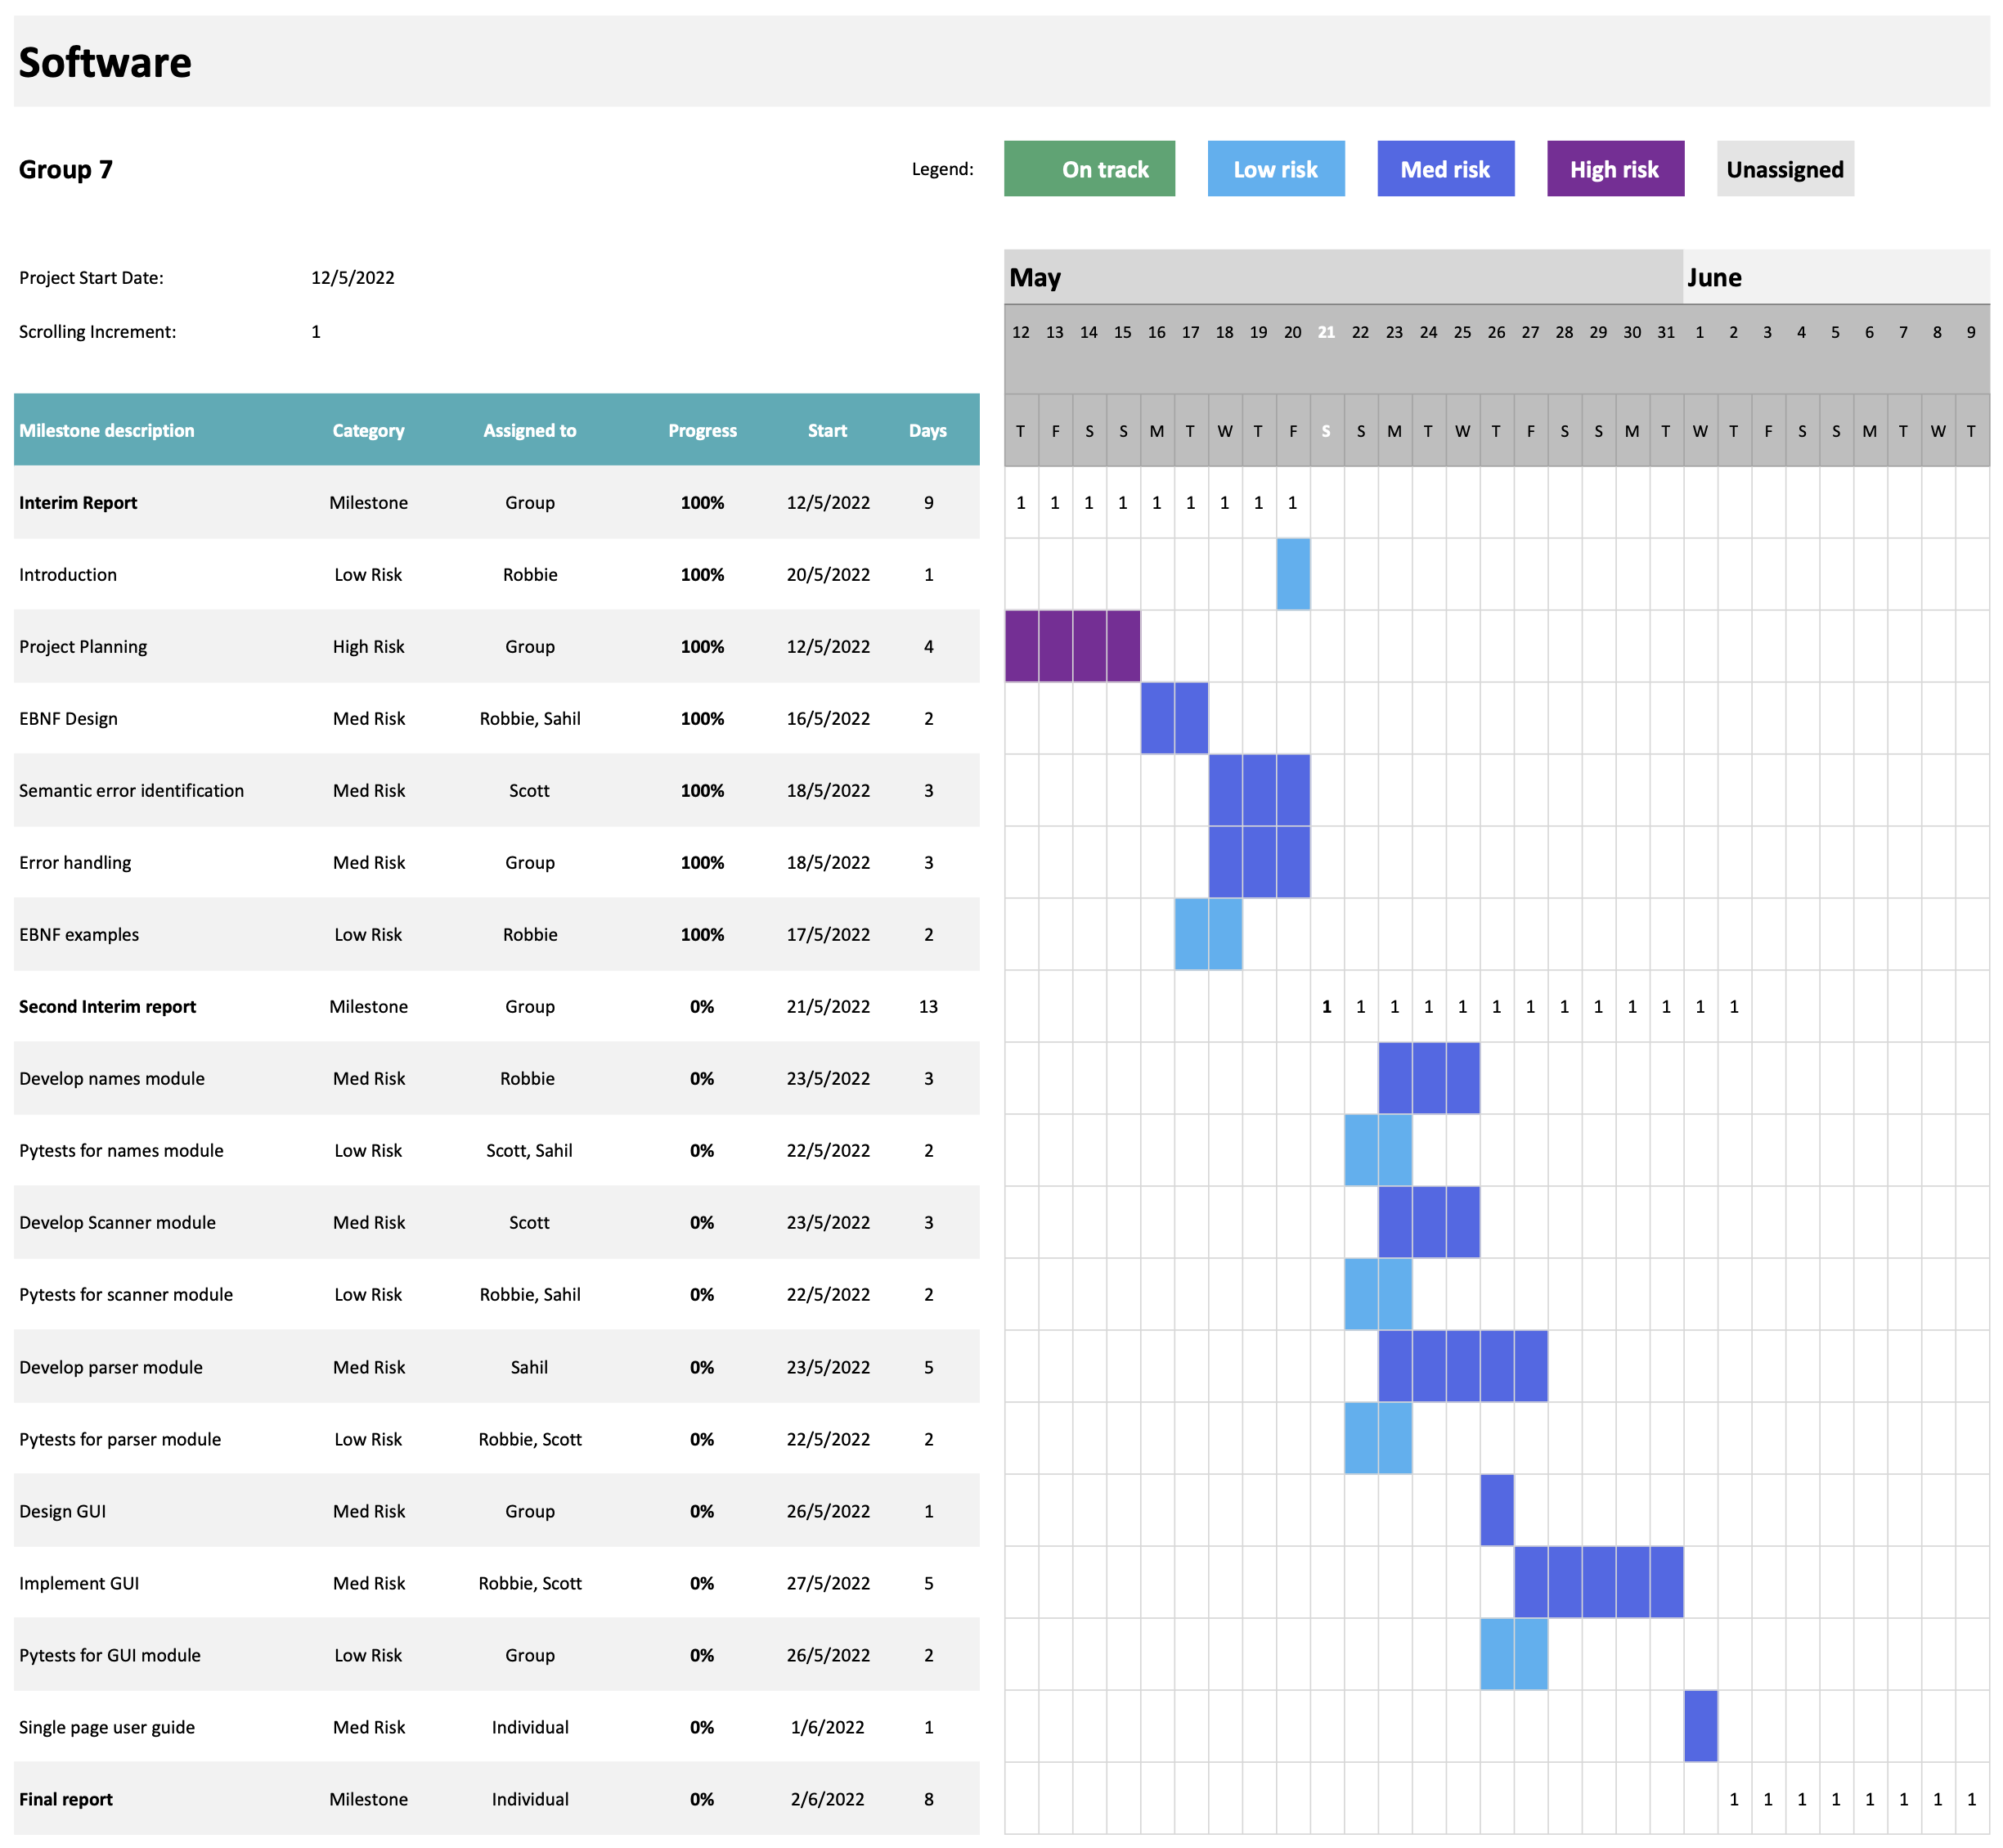
\includegraphics[width=\linewidth]{Gantt.png}
  \caption{Gantt Chart}
\end{figure}

\newpage
\section{EBNF syntax design}
Our approach to EBNF syntax design consisted of putting together a rough first attempt and then iterating the design to improve the readability, length and error handling while ensuring it conforms to LL(1) grammar. One of the first design choices we were encountered with was to decide if it was mandatory to define at least one monitor point. Ultimately we decided it should be since the purpose of the software is to monitor points on the logic circuit and so it is more likely a user would forget to define one and not understand why there were not getting any signals being outputted. \\

At this stage we had a rough first version and we began the iteration process.  At first we had circuit elements defined in the following way 

\begin{verbatim}
"SW1" = SWITCH - OFF
"SW2" = SWITCH - OFF,
\end{verbatim}

We decided however the speech marks were not necessary as the way the grammar is set up there is no real need to distinguish between keywords and names as the grammar will know what to expect. That being said, we still decided to not allow variable names to be named as keywords as it would make the file less readable and potentially more confusing even though there are no syntactic implications. We also decided that we should aim to make the syntax as familiar as possible as it would make it easier to read and reduce the learning curve to writing definition files. We hence decided to create devices in a object initialiser format giving: 

\begin{verbatim}
SW1 = SWITCH(OFF),
SW2 = SWITCH(OFF)
\end{verbatim}

This way is more familiar to defining an object of type switch and passing in any necessary parameters. \\

The next upgrade we considered was making sure the file could be readable in a number of different formats, since all white spaces and line breaks are removed; the definition could in theory be written on one line. Hence we decided to replace

\begin{verbatim}
circuit  = "CIRCUIT", ":", devices, connections, monitors;
\end{verbatim}

with

\begin{verbatim}
circuit  = CIRCUIT, '\{', devices, connect, monitors, '\}';
\end{verbatim}

Similar changes were made to devices, connections and monitors. The use of the braces allows unambiguous one line circuit definition files.The use of braces also allows different stopping symbols to be used, this has the advantage of being able to skip less when the parser is picking up errors.\\

The last main modification we decided to make is to define multiple device elements of the same type in one line.

\begin{verbatim}
SW1, SW2, SW3 = SWITCH(OFF);
G1, G3 = XOR;
\end{verbatim}

This allows definition files to be more condensed. This also meant we had to replace the end of a device definition with a semicolon instead of a comma, having these separate stopping symbols again helps to decide how much code to skip when error checking. \\

\newpage
\subsection{Language definition file}

\begin{verbatim}
network = circuit, "END";

circuit  = "CIRCUIT", "{", devices, connections, monitorlist, "}";

devices = "DEVICES", "{", device, { device }, "}";

device = devicename, {",", devicename}, "=",  ( clock | switch | and | nand | or | nor | dtype | xor), ";";

name = letter, { character };

clock = "CLOCK", "(", number, ")";

number = nonzerodigit, { digit };

switch = "SWITCH", "(", ( "ON" | "OFF" ), ")";

and = "AND", "(", number, ")";

nand = "NAND", "(", number, ")";

or = "OR", "(", number, ")";

nor = "NOR", "(", number, ")";

dtype = "DTYPE";

xor = "XOR";

character = letter | digit;

connections = "CONNECT", "{", con, { con }, "}";

con = point, ">", point, {",", point}, ";";

point = devicename, [".", pinname];

devicename = name;

pinname = name;

monitorlist = "MONITOR", "{", monitor, { monitor }, "}";

monitor = point, ";";
\end{verbatim}


\newpage
\subsection{Example definition files}

\subsubsection{Example 1}

\begin{figure}[H]
\centering
\captionsetup{justification = centering}
  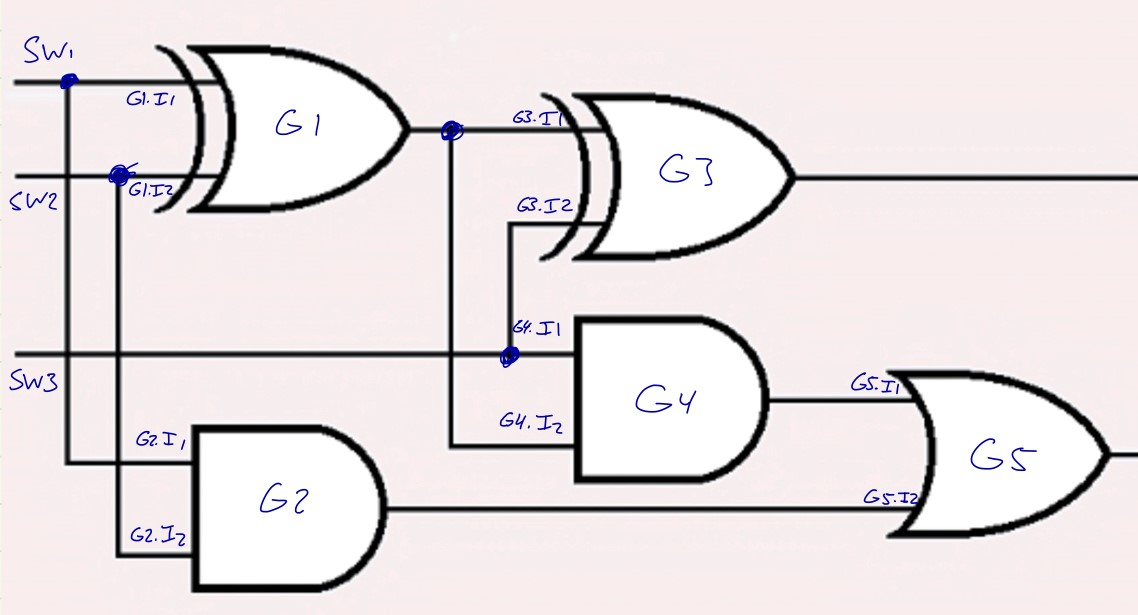
\includegraphics[width=0.5\linewidth]{Example2CircuitDiagram.jpg}
  \caption{Circuit 1}
\end{figure}

\begin{verbatim}
CIRCUIT
{

DEVICES
{
    SW1, SW2, SW3 = SWITCH(OFF);
    G1, G3 = XOR;
    G2, G4 = AND(2);
    G5 = OR(2);
}

CONNECT
{
    SW1 > G1.I1, G2.I1;
    SW2 > G1.I2, G2.I2;
    SW3 > G3.I2, G4.I1;
    G1 > G3.I1, G4.I2;
    G2 > G5.I2;
    G4 > G5.I1;
}

MONITOR
{
    G3;
    G5;
    SW1;
    SW2;
    SW3;
}

}

END
\end{verbatim}

\newpage
\subsubsection{Example 2}

\begin{figure}[H]
\centering
\captionsetup{justification = centering}
  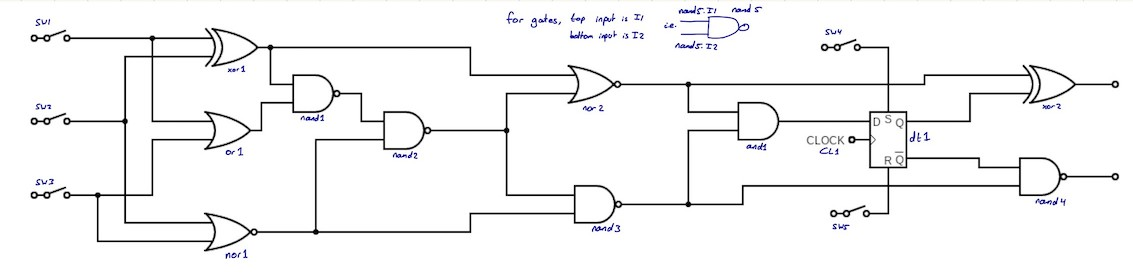
\includegraphics[width=\linewidth]{Example3CircuitDiagram.jpg}
  \caption{Circuit 2}
\end{figure}

\begin{verbatim}
CIRCUIT
{

DEVICES
{
    SW1, SW2, SW3, SW4, SW5 = SWITCH(OFF);
    nand1, nand2, nand3, nand4 = NAND(2);
    nor1, nor2 = NOR(2);
    xor1, xor2 = XOR;
    or1 = OR(2);
    and1 = AND(2);
    CL1 = CLOCK(20);
    dt1 = DTYPE;
}

CONNECT
{
    SW1 > xor1.I1, or1.I1;
    SW2 > xor1.I2, nor1.I1;
    SW3 > or1.I2, nor1.I2;
    xor1 > nand1.I1, nor2.I2;
    or1 > nand1.I2;
    nor1 > nand2.I2, nand3.I2;
    nand1 > nand2.I1;
    nand2 > nor2.I2, nand3.I1;
    nor2 > and1.I1, xor2.I1;
    nand3 > and1.I2, nand4.I2;
    and1 > dt1.DATA;
    CL1 > dt1.CLK;
    SW4 > dt1.SET;
    SW5 > dt1.CLEAR;
    dt1.Q > xor2.I2;
    dt1.QBAR > nand4.I1;
}

MONITOR
{
    xor2; nand4;
}

}

END
\end{verbatim}

\newpage
\section{Identification of all possible semantic errors}

Syntax errors are quite simple to detect for a parser of an LL(1) language. Semantic errors are a lot harder to detect. Each semantic error is an error in the logic of the file and therefore it is hard to think of all the errors that could occur. With our syntax, there are five types of semantic error that can occur in the definition file. \\

The first is if a connection is not between an output and an input. This leads to two subcategories, where either two inputs are connected to each other or two outputs are connected. \\

Another error relating to the connecting of the devices occurs when either multiple or zero outputs are connected to an input pin because an input must have exactly one output connected to it. \\

According to our EBNF grammar, a connection can be made from a pin with any name belonging to a device with any name. However, for this to make logical sense, the pin and device in question must have been defined in the “DEVICES” section because to make a connection the points to be connected must exist.\\

There are also some limitations on the arguments when creating devices. The logic gates (excluding XOR) must have a number of inputs in the range 1-16. A creation of a gate AND(17) would therefore be an error.\\

The final semantic error is that a device or pin name cannot be one of the keywords in the definition file (e.g. “CIRCUIT”, “DEVICES”, ...). This would cause the parser to break down as it would enter into a different rule of the grammar and expect a different object to follow.

\section{Description of error handling}

There are two types of error that need to be detected and reported to the user, these are syntax errors and semantic errors. Both of these errors are detected and reported by the parser module. Syntax errors will be flagged as the parser receives the symbols one by one from the scanner and checks that the symbols conform to the defined EBNF grammar by having a function for each rule. We aim to then report this error to the user with the exact location of the error, we will achieve this by augmenting the symbol class to include the line number and location of the symbol. The error handler will store the current character location and when an error occurs will print the characters in that part of the circuit definition file leaving a line in between lines if the error occurs over multiple lines and then place a pointer to the exact location of the error. \\

Alongside this we would also like to give as much information about what we think they could have meant or if they missed a symbol. We can do this by also reporting the next symbol the parser was expecting to receive (e.g. if they are defining a device and try create a device that does not exist, we give a list of supported devices). We have also given some thought to special cases and useful error messages we can give in these cases but these ideas will only be implemented if time permits. An example would be forgetting to put a comma when defining multiple identical devices eg SW1 SW2 = SWITCH(OFF) which would create a device with name SW1SW2, this would only flag an error once they are told that SW1 does not exist when attempting to make a connection including the SW1 device. It will not be clear to the user why it does not exist. The idea is to look at what connection they are attempting to make and check if the device is a prefix of an existing device in which case we could suggest that they may have meant SW1 , SW2. This we recognise is far from a perfect solution but could be more helpful in certain cases. \\

Semantic errors will be handled by attempting to construct the network while parsing and then if any semantic issues occur then this is reported by the relevant modules and then this is passed to the user. Again the full line where the error occurred will be reported but this time the semantic issue will be stated. If a semantic issue does occur we will stop building the network any further and the parser will resume from the next stopping symbol, this means that no further semantic errors will be picked up but any syntax errors will be, this is sensible since for example if a device is not defined but then referred to multiple times throughout the definition file it will get flagged up multiple times even though it was just one error really, where as syntax errors are more standalone. An error count will also be kept and reported to the user.

\end{document}
